\scanpage{59}
\uline{Compléments sur les groupes de Witt}

\uline{Lemme 1}\quad Soit $S=\operatorname{Spec}(A)$ de car. $p$.
\deleted{Posons $\unsure{A[F]=\mathbb F_p[F}$}
$\operatorname{Ext}^1(G_a,G_a)$ est le
\deleted{$A[F]$-module} $A$-module libre engendré par les
$\unsure{F_*^i}e$,
\inserted{i.e. le $A[F]$-module libre
\inserted{\figure{\begin{tikzpicture}
\node[draw,ellipse] {\uuline{à gauche}};
\end{tikzpicture}}}
engendré par $e$,}
où $e$ est la classe de $W_2$ considéré comme extension de $G_a$ par $G_a$.
\figure{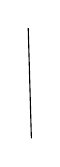
\begin{tikzpicture}\draw (0,0)--(.04,-1.4);\end{tikzpicture}}

\uline{Dém}\quad On peut supposer, par linéarité, que $A=\mathbb F_p$.
Mais c'est fait dans Demazure--Gabriel, II \S 3 4.6

\uline{Lemme 2}\quad Soit $H$ un sous-schéma en groupes de $G_a$, tel
\deleted{\unsure{fini}} que l'on ait $H\simeq G_a$, ou
\inserted{$H$ est fini loc. libre sur $S$,}
\deleted{\unsure{que $G/H$ est}}
$G/H$ est loc. isom. à $G_a$ (pour fppf).
Alors on a

a) $\underline{\operatorname{Ext}}^1(H,W_n)
\xrightarrow{R_*^{n-1}}\operatorname{Ext}^1(H,W_1)$ est bijection,

i.e. \deleted{$\unsure{V}\operatorname{Ext}^1(H,W_{n-1})
-\operatorname{Ext}^1(H,W_n)$ est nulle i.e.}
\deleted{$\unsure{\operatorname{Ext}}$}

\[
\begin{aligned}
a_1)\quad&
\operatorname{Ext}^1(H,W_{n-1})\xrightarrow{V}\operatorname{Ext}^1(H,W_n)
\quad\text{est nulle, i.e.}\\
&\operatorname{Hom}(H,G_a)-\operatorname{Ext}^1(H,W_{n-1})
\quad\text{est surjectif}\\
a_2)\quad&
\operatorname{Ext}^1(H,W_1)\longrightarrow\operatorname{Ext}^1(H,W_{n-1})
\quad\text{est nulle}
\end{aligned}
\]

b) $\operatorname{Ext}^1(G_a,W_n)-\operatorname{Ext}^1(H,W_n)$
\uline{surjective}

(i.e. $\operatorname{Ext}^1(H,W_n)-\operatorname{Ext}^2(G_a/H,W_n)$
est nulle)

c) $\underline{\operatorname{Ext}}^1(G_a,W_n)$ est un $A[F]$-module
\deleted{libre de base la}
\inserted{\uuline{à droite}, engendré par la}
classe \deleted{\unsure{e}} de $W_{n+1}$.

\uline{Dém}\quad \uline{$n=1$}\quad Alors a) est trivial,
b) résulte de $\underline{\operatorname{Ext}}^2(G_a/H,W_1)=0$
(qui résulte, par dévissage sur $n$ et descente fppf, de
$\underline{\operatorname{Ext}}^2(G_a,G_a)=0$)
et c) n'est autre que le lemme 1.

\inserted{\uline{$n$ général:}}
On procède comme dans \deleted{\unsure{le}} loc. cit.
\inserted{V \S 1 2.2.}, par récurrence sur $n$.
\margin{69}
